\section{Matrix Algebra}\label{sec:Matrix_Algebra}
\begin{definition}[Matrix]\label{def:Matrix}
  A \emph{matrix} is an array of numbers subject to special addition and multiplication rules.
  They are represented with capital letters, $A$, $B$, etc.
  However, other texts may bold those capital letters to, $\mathbf{A}$, $\mathbf{B}$, etc.
  When written, they can be written in one of two ways, but they both mean the same thing.
  \begin{equation}\label{eq:Matrix}
    \begin{aligned}
      &\begin{pmatrix}
        a_{11} & a_{12} \\
        a_{21} & a_{22} \\
      \end{pmatrix} \\
      &\begin{bmatrix}
        a_{11} & a_{12} \\
        a_{21} & a_{22} \\
      \end{bmatrix}
    \end{aligned}
  \end{equation}
\end{definition}

Matrices are very useful, as learning the intricacies of them allows for quick solving of larger problems.

\subsection{Properties of Matrices}\label{subsec:Properties_Matrices}
\subsubsection{Properties of Matrix Addition}\label{subsubsec:Properties_Matrix_Addition}
\begin{propertylist}
\item \nameref{def:Matrix} Addition is commutative.\label{prop:Matrix_Add_Commutative}
  \begin{equation}\label{eq:Matrix_Add_Commutative}
    A+B = B+A
  \end{equation}

\item \nameref{def:Matrix} Addition is associative.\label{prop:Matrix_Add_Associative}
  \begin{equation}\label{eq:Matrix_Add_Associative}
    A+(B+C) = (A+B) + C
  \end{equation}

\item For any \nameref{def:Matrix} $A$, there is a unique matrix, $I$ or $O$, such that the equation below holds true.\label{prop:Matrix_Additive_Identity}
  \begin{equation}\label{eq:Matrix_Additive_Identity}
    A+O = A
  \end{equation}

\item For each \nameref{def:Matrix} $A$, there is a unique matrix $-A$ such that the equation below holds true.\label{prop:Matrix_Additive_Inverse}
  \begin{equation}\label{eq:Matrix_Additive_Inverse}
    A+(-A) = O
  \end{equation}

\item $A+B$ is a \nameref{def:Matrix} of the same dimensions as $A$ and $B$.\label{prop:Matrix_Addition_Closure}
\end{propertylist}

\subsubsection{Properties of Matrix Multiplication}\label{subsubsec:Properties_Matrix_Multiplication}
Matrix multiplication is defined as follows:
\begin{equation}\label{eq:Matrix_Multiplication}
  \begin{bmatrix}
    a_{11} & a_{12} & a_{13} & \cdots & a_{1n} \\
    a_{21} & a_{22} & \ddots & \ddots & a_{2n} \\
    \vdots & \ddots & \ddots & \ddots & a_{mn} \\
    a_{n\,1} & a_{n\,2} & \cdots & \cdots & a_{nn}
  \end{bmatrix}
\end{equation}

\begin{propertylist}
\item In general, \nameref{def:Matrix} multiplication is \textbf{NOT} commutative.\label{prop:Matrix_Not_Commutative}
  \begin{equation}\label{eq:Matrix_Mult_Not_Commutative}
    AB \neq BA
  \end{equation}

\item \nameref{def:Matrix} multiplication is associative.\label{prop:Matrix_Associativity}
  \begin{equation}\label{eq:Matrix_Mult_Associativity}
    (AB) C = A (BC)
  \end{equation}
\item \nameref{def:Matrix} multiplication is distributive.\label{prop:Matrix_Distributivity}
  \begin{equation}\label{eq:Matrix_Mult_Distributivity}
    \begin{aligned}
      A (B+C) &= AB + AC \\
      (B+C) A &= BA + CA
    \end{aligned}
  \end{equation}

\item There exists a \nameref{def:Matrix} $I$ that forms the \nameref{def:Multiplicative_Identity_Matrix} that satisfies the following rule:\label{prop:Mult_Identity_Matrix}
  \begin{equation}\label{eq:Mult_Identity_Matrix}
    \begin{aligned}
      AI &= A \\
      IA &= A
    \end{aligned}
  \end{equation}
  \begin{remark*}
    This is one of the two general cases where \nameref{def:Matrix} multiplication \textbf{IS} commutative.
  \end{remark*}

\item There exists a \nameref{def:Matrix} $O$ that forms the \nameref{def:Zero_Matrix}, satisfying the following rule:\label{prop:Mult_Zero_Matrix}
  \begin{equation}\label{eq:Mult_Zero_Matrix}
    \begin{aligned}
      AO &= O \\
      OA &= O
    \end{aligned}
  \end{equation}
  \begin{remark*}
    This is one of the two general cases where \nameref{def:Matrix} multiplication \textbf{IS} commutative.
  \end{remark*}

\item When performing multiplication, the \textbf{dimension property} states that the product of an $m \by n$ and an $n \by k$ matrix is an $m \by k$ \nameref{def:Matrix}.\label{prop:Mult_Dimension_Property}
\end{propertylist}

\begin{definition}[Identity Matrix]\label{def:Multiplicative_Identity_Matrix}
  The \emph{identity matrix}, $I$ is one that satisfies \Cref{prop:Mult_Identity_Matrix}.
  These follow the forms of the ones shown below.
  \begin{equation}\label{eq:Multiplicative_Identity_Matrix}
    \begin{aligned}
      I &=
      \begin{bmatrix}
        1 & 0 \\
        0 & 1 \\
      \end{bmatrix} \\
      &=
      \begin{bmatrix}
        1 & 0 & 0 \\
        0 & 1 & 0 \\
        0 & 0 & 1 \\
      \end{bmatrix}
    \end{aligned}
  \end{equation}
\end{definition}

\begin{definition}[Zero Matrix]\label{def:Zero_Matrix}
  The \emph{zero matrix}, $O$, is one that satisfies \Cref{prop:Mult_Zero_Matrix}.
  For \nameref{def:Matrix} multiplication, it is a matrix of all $0$.
  \begin{equation}
    \label{eq:3}
    \begin{aligned}
      O &=
      \begin{bmatrix}
        0 & 0 \\
        0 & 0 \\
      \end{bmatrix} \\
      &=
      \begin{bmatrix}
        0 & 0 & 0 \\
        0 & 0 & 0 \\
        0 & 0 & 0 \\
      \end{bmatrix}
    \end{aligned}
  \end{equation}
\end{definition}

%%% Local Variables:
%%% mode: latex
%%% TeX-master: "../../Math_333-MatrixAlg_ComplexVars-Reference_Sheet"
%%% End:


\subsection{Systems of Equations}\label{subsec:Systems_Equations}
A \nameref{def:Matrix} can be used to represent a system of equations.

For example,
\begin{align*}
  x + 2y + 3z &= 5 \\
  2x - y + z &= 3 \\
  x - y + 5z &= 2
\end{align*}
can be represented with a set of matrices as follows
\begin{equation*}
  \begin{bmatrix}
    1 & 2 & 3 \\
    2 & -1 & 1 \\
    1 & -1 & 5 \\
  \end{bmatrix}
  \begin{bmatrix}
    x \\
    y \\
    z \\
  \end{bmatrix}
  =
  \begin{bmatrix}
    5 \\
    3 \\
    2 \\
  \end{bmatrix}
\end{equation*}


%%% Local Variables:
%%% mode: latex
%%% TeX-master: "../../Math_333-MatrixAlg_ComplexVars-Reference_Sheet"
%%% End:


\subsection{Elementary Row Operations}\label{subsec:Elementary_Row_Ops}

%%% Local Variables:
%%% mode: latex
%%% TeX-master: "../../Math_333-MatrixAlg_ComplexVars-Reference_Sheet"
%%% End:


\subsection{Echelon Form}\label{subsec:Echelon_Form}

%%% Local Variables:
%%% mode: latex
%%% TeX-master: "../../Math_333-MatrixAlg_ComplexVars-Reference_Sheet"
%%% End:


\subsection{Gaussian Elimination}\label{subsec:Gaussian_Elimination}
\begin{definition}[Gaussian Elimination]\label{def:Gaussian_Elimination}
  \emph{Gaussian elimination} is a method of solving a system of linear equations using matrices and \nameref{def:Elementary_Row_Op}s.
\end{definition}

It is easier to show how \nameref{def:Gaussian_Elimination} works through an example.

\begin{example}[Lecture 12, Example 3]{Perform Gaussian Elimination}
  Solve the system of linear equations below.
  \begin{align*}
    x - 2y + 3z &= 5 \\
    2x + y - z &= 8 \\
    3x - y + 2z &= 13
  \end{align*}
  \tcblower{}
  Start by converting the system of linear equations to an \nameref{def:Augmented_Matrix}.
  \begin{align*}
    \begin{array}{cccl}
      1x &- 2y &+ 3z &= 5 \\
      2x &+ 1y &- 1z &= 8 \\
      3x &- 1y &+ 2z &= 13 \\
    \end{array}
         &=
           \begin{amat}{3}
             1 & -2 & 3 & 5 \\
             2 & 1 & -1 & 8 \\
             3 & -1 & 2 & 13 \\
           \end{amat} \\
    \intertext{Use repeated \nameref{def:Elementary_Row_Op}s to make lower rows have zeros, converting to \nameref{thm:Echelon_Form}.}
         &\grstep{-2r_{1}+r_{2}}\begin{amat}{3}
           1 & -2 & 3 & 5 \\
           0 & 5 & -7 & -2 \\
           3 & -1 & 2 & 13 \\
         \end{amat} \\
         &\grstep{-3r_{1}+r_{3}}\begin{amat}{3}
           1 & -2 & 3 & 5 \\
           0 & 5 & -7 & -2 \\
           0 & 5 & -7 & -2 \\
         \end{amat} \\
         &\grstep{\frac{1}{5}r_{2}}\begin{amat}{3}
           1 & -2 & 3 & 5 \\
           0 & 1 & \frac{-7}{5} & \frac{-2}{5} \\
           0 & 5 & -7 & -2 \\
         \end{amat} \\
         &\grstep{-5r_{2}+r_{3}}\begin{amat}{3}
           1 & -2 & 3 & 5 \\
           0 & 1 & \frac{-7}{5} & \frac{-2}{5} \\
           0 & 0 & 0 & 0 \\
         \end{amat} \\
  \end{align*}

  Now, we can reconvert back into a system of linear equations.
  \begin{equation*}
    \begin{amat}{3}
      1 & -2 & 3 & 5 \\
      0 & 1 & \frac{-7}{5} & \frac{-2}{5} \\
      0 & 0 & 0 & 0 \\
    \end{amat} \\
    =
    \begin{array}{cccl}
      1x &- 2y &+ 3z &= 5 \\
      0x &+ 1y &- \frac{7}{5}z &= \frac{-2}{5} \\
      0x &+ 0y &+ 0z &= 0 \\
    \end{array}
  \end{equation*}

  We now have 3 unknowns, but only 2 usable equations.
  Therefore, we solve for two of the unknowns in terms of a third.
  \begin{align*}
    y &= \frac{-2}{5} + \frac{7}{5}z \\
    x &= \frac{21}{5} - \frac{z}{5}
  \end{align*}
\end{example}

\begin{definition}[Consistent]\label{def:Consistent}
  A \emph{consistent} system of linear equations is one which has a solution.
\end{definition}


%%% Local Variables:
%%% mode: latex
%%% TeX-master: "../../Math_333-MatrixAlg_ComplexVars-Reference_Sheet"
%%% End:


\subsection{Elementary Matrix Operations}\label{subsec:Elementary_Matrix_Ops}
\begin{definition}[Elementary Matrix]\label{def:Elementary_Matrix}
  An \emph{elementary matrix} is a \nameref{def:Matrix} obtained by performing an \nameref{def:Elementary_Row_Op} on the \nameref{def:Multiplicative_Identity_Matrix}.
  This allows us to encode the action we take on the identity matrix \textbf{into} the identity matrix, essentially saving it.
\end{definition}

\begin{blackbox}
  Given the \nameref{def:Multiplicative_Identity_Matrix}, $I$, a regular \nameref{def:Matrix} $A$, perform a row reduction by adding $r_{1}$, multiplied by $\lambda$, of $A$ to $r_{2}$.
  \begin{align*}
    I &= \begin{bmatrix}
      1 & 0 \\
      0 & 1
    \end{bmatrix} \\
    A &= \begin{bmatrix}
      a_{11} & a_{12} \\
      a_{21} & a_{22}
    \end{bmatrix}
  \end{align*}

  We perform the \nameref{def:Elementary_Row_Op} on the \nameref{def:Multiplicative_Identity_Matrix}.
  \begin{equation*}
    \begin{bmatrix}
      1 & 0 \\
      0 & 1
    \end{bmatrix}
    \grstep{\lambda r_{1}+r_{2}}
    \begin{bmatrix}
      1 & 0 \\
      \lambda & 1
    \end{bmatrix}
  \end{equation*}

  Now that we have an \nameref{def:Elementary_Matrix}, we can perform the action we saved in the elementary matrix on any matrix, in this case, $A$.
  \begin{equation*}
    \begin{bmatrix}
      1 & 0 \\
      \lambda & 1
    \end{bmatrix}
    \begin{bmatrix}
      a_{11} & a_{12} \\
      a_{21} & a_{22}
    \end{bmatrix}
    =
    \begin{bmatrix}
      a_{11} & a_{12} \\
      \lambda a_{11} + a_{21} & \lambda a_{12} + a_{22}
    \end{bmatrix}
  \end{equation*}

  We can see that this result is the exact same as if we have performed the \nameref{def:Elementary_Row_Op} on the matrix $A$ directly.
\end{blackbox}


%%% Local Variables:
%%% mode: latex
%%% TeX-master: "../../Math_333-MatrixAlg_ComplexVars-Reference_Sheet"
%%% End:


\subsection{Inverse Matrices}\label{subsec:Inverse_Matrices}

%%% Local Variables:
%%% mode: latex
%%% TeX-master: "../../Math_333-MatrixAlg_ComplexVars-Reference_Sheet"
%%% End:


\subsection{Reduced Row Echelon Form}\label{subsec:RREF}
Using what we learned in \Cref{subsec:Inverse_Matrices} and \Cref{subsubsec:Inverse_Matrices_using_Elementary_Matrices}, we can solve systems of linear equations using a \nameref{def:Matrix}'s inverse.

This can be movtivated with a general example.
\begin{blackbox}
  Consider the system shown below.
  \begin{align*}
    a_{11} x_{1} + a_{12} x_{2} &= b_{1} \\
    a_{21} x_{1} + a_{22} x_{2} &= b_{2}
  \end{align*}

  We can convert this set of equations with 2 equations and 2 unknowns to a single linear equation with a single unknown.
  \textbf{Equivalently} to the system, we can write
  \begin{align*}
    \begin{pmatrix}
      a_{11} & a_{12} \\
      a_{21} & a_{22}
    \end{pmatrix}
    \begin{pmatrix}
      x_{1} \\
      x_{2}
    \end{pmatrix} &=
    \begin{pmatrix}
      a_{11} x_{1} + a_{12} x_{2} \\
      a_{21} x_{1} + a_{22} x_{2}
    \end{pmatrix} \\
    &=
      \begin{pmatrix}
        b_{1} \\
        b_{2}
      \end{pmatrix}
  \end{align*}

  The column matrices (column vectors) are technically one unknown with multiple unknown components.

  Just like with regular algebra, we can use the inverse of the items we know to solve the equation.
  \begin{align*}
    \intertext{Let}
    A &=
        \begin{pmatrix}
          a_{11} & a_{12} \\
          a_{21} & a_{22}
        \end{pmatrix} \\
    X &=
        \begin{pmatrix}
          x_{1} \\
          x_{2}
        \end{pmatrix} \\
    B &=
        \begin{pmatrix}
          b_{1} \\
          b_{2}
        \end{pmatrix} \\
    AX &= B \\
    \shortintertext{We make the assumption $A$ is invertible.}
    A^{-1} (A X) &= A^{-1} B \\
    (A^{-1} A) X &= A^{-1} B \\
    I X &= A^{-1} B
  \end{align*}

  Therefore, we can solve the system using $A^{-1}$.
\end{blackbox}


%%% Local Variables:
%%% mode: latex
%%% TeX-master: "../../Math_333-MatrixAlg_ComplexVars-Reference_Sheet"
%%% End:


\subsection{Linear Independence}\label{subsec:Linear_Independence}
\begin{theorem}[Linearly Dependent]\label{thm:Linearly_Dependent}
  Let $S$ be a set of vectors of size $n$, $S = \lbrace v_{1}, v_{2}, \ldots, v_{n} \rbrace$.
  Each vector $v_{k}$ has components in $\RealNumbers^{m}$ ($m$ components from $\RealNumbers$).

  The set is \emph{linearly dependent} if there exists scalars $c_{1}, c_{2}, \ldots, c_{n}$, at least one of which is not equal to zero, such that the below equation holds true.
  \begin{equation}\label{eq:Linearly_Dependent}
    c_{1}v_{1} + c_{2}v_{2} + \cdots + c_{n}v_{n} = 0
  \end{equation}

  \begin{remark*}
    Note that the $0$ in \Cref{eq:Linearly_Dependent} implies the zero vector, not necessarily the scalar value $0$.
  \end{remark*}
\end{theorem}


%%% Local Variables:
%%% mode: latex
%%% TeX-master: "../../Math_333-MatrixAlg_ComplexVars-Reference_Sheet"
%%% End:


\subsection{Matrix Rank}\label{subsec:Matrix_Rank}
\begin{definition}[Rank]\label{def:Matrix_Rank}
  The \emph{rank} of a \nameref{def:Matrix} $A_{n \by m}$ is the largest number of \nameref{def:Linearly_Independent} ``chunks'' of a matrix.

  There are 2 kinds of rank: \nameref{rmk:Row_Rank} and \nameref{rmk:Column_Rank}.

  \begin{remark}[Row Rank]\label{rmk:Row_Rank}
    The \emph{rank} of a \nameref{def:Matrix} $A_{n \by m}$ is the largest number of \nameref{def:Linearly_Independent} rows of a matrix.
  \end{remark}

  \begin{remark}[Column Rank]\label{rmk:Column_Rank}
    The \emph{column rank} of a \nameref{def:Matrix} $A_{n \by m}$ is the largest number of \nameref{def:Linearly_Independent} columns of a matrix.
  \end{remark}

  \begin{remark}[Row Rank Column Rank Equivalence]
    \nameref{rmk:Row_Rank} can be proven to be the same as the \nameref{rmk:Column_Rank} for all matrices.
  \end{remark}
\end{definition}

%%% Local Variables:
%%% mode: latex
%%% TeX-master: "../../Math_333-MatrixAlg_ComplexVars-Reference_Sheet"
%%% End:


\subsection{Determinants}\label{subsec:Determinants}
Before calculating the \nameref{def:Determinant}, we need to have some additional vocabulary wto work with.

\begin{definition}[Minor]\label{def:Minor}
  The \emph{minor} $\Minor{i}{j}$ is the \nameref{def:Determinant} of the sub\nameref{def:Matrix} obtained by deleting the $i$th row and $j$th column.
\end{definition}

\begin{blackbox}
  Given the matrix $
  \begin{pmatrix}
    1 & -1 & 3 \\
    2 & 5 & -1 \\
    3 & 0 & 5
  \end{pmatrix}$, the \nameref{def:Minor} at the index $3,2$ is found by deleting the \nth{3} row and \nth{2} column and taking the \nameref{def:Determinant} of the resulting submatrix.
  Thus,
  \begin{align*}
    \Minor{3}{2} &= \det
                   \begin{pmatrix}
                     1 & 3 \\
                     2 & -1
                   \end{pmatrix} \\
    \intertext{Use the definition of the \nameref{def:Determinant} for a $2 \by 2$ \nameref{def:Matrix}.}
                 &= 1(-1) - 3(2) \\
                 &= -1 - 6 \\
                 &= -7
  \end{align*}
\end{blackbox}

\begin{definition}[Cofactor]\label{def:Cofactor}
  The \emph{cofactor} $\Cofactor{i}{j}$ is related to the \nameref{def:Minor}, $\Minor{i}{j}$ by the equation below.
  \begin{equation}\label{eq:Cofactor}
    \Cofactor{i}{j} = {(-1)}^{i + j} \Minor{i}{j}
  \end{equation}
\end{definition}

\begin{blackbox}
  Using the same \nameref{def:Matrix} from earlier, the \nameref{def:Cofactor} of of the element in the \nth{3} row and \nth{2} column is:
  \begin{align*}
    \Cofactor{3}{2} &= {(-1)}^{3+2} \Minor{3}{2} \\
                    &= (-1) (-7) \\
                    &= 7
  \end{align*}
\end{blackbox}

Now with these terms defined, we can define the general algorithm for the \nameref{def:Determinant}.

\begin{definition}[Determinant]\label{def:Determinant}
  The \emph{determinant} of a \nameref{def:Matrix} is a scalar value that is computed out of a \textbf{square} matrix and encodes certain properties of the transformation specified by the matrix.

  There are 2 equations in use for the determinant, depending on the size of the matrix.
  For a $2 \by 2$ matrix,
  \begin{equation}\label{eq:Determinant_2x2}
    \det
    \begin{pmatrix}
      a & b \\
      c & d
    \end{pmatrix}
    = ad - bc
  \end{equation}

  For a matrix larger than $2 \by 2$, we have many possible ways of finding the determinant.
  This is explored further in \Cref{subsubsec:Expand_Determinant}, with their equations given in \Cref{eq:Determinant_Expand_ith_Row} and \Cref{eq:Determinant_Expand_jth_Column}.
\end{definition}


%%% Local Variables:
%%% mode: latex
%%% TeX-master: "../../Math_333-MatrixAlg_ComplexVars-Reference_Sheet"
%%% End:


\subsection{Eigenvectors}\label{subsec:Eigenvectors}
\begin{definition}[Eigenvector]\label{def:Eigenvector}
  Let $A$ be an $n \by n$ matrix, denoted $A_{n \by n}$ and $X_{n \by 1}$ be a column vector of unknowns.
  $X_{n \by 1}$ is said to be an \emph{eigenvector} of $A$ if:

  \begin{equation}\label{eq:Eigenvector}
    AX = \lambda X
  \end{equation}

  \begin{propertylist}
  \item $X \neq 0$.\label{prop:Eigenvector_Nonzero}
  \item $\lambda$ is a scalar, called an \nameref{def:Eigenvalue}.\label{prop:Eigenvector_Value}.
  \end{propertylist}

  \begin{remark}[Uniqueness of Eigenvectors]
    There can be infinitely many \nameref{def:Eigenvector}s for a given \nameref{def:Eigenvalue}.
  \end{remark}
\end{definition}

\begin{example}[Lecture 17, Example 1]{Verify Vector is not an Eigenvector}
  Given $A$ and $Y$, is $Y$ an \nameref{def:Eigenvector} of $A$?
  \begin{align*}
    A &=
        \begin{pmatrix}
          2 & 3 \\
          6 & -1
        \end{pmatrix} &
                        Y &=
                            \begin{pmatrix}
                              2 \\
                              -1
                            \end{pmatrix}
  \end{align*}
  \tcblower{}
  First, we check that the two properties of an \nameref{def:Eigenvector} are satisfied.
  \Cref{prop:Eigenvector_Nonzero} is satisfied ($Y \neq 0$).

  Now, we attempt to find the \nameref{def:Eigenvalue} for this particular \nameref{def:Eigenvector}.
  \begin{align*}
    AY &=
         \begin{pmatrix}
           2 & 3 \\
           6 & -1
         \end{pmatrix}
               \begin{pmatrix}
                 2 \\
                 -1
               \end{pmatrix} \\
    &=
      \begin{pmatrix}
        1 \\
        13
      \end{pmatrix} \\
  \end{align*}

  The problem here is that there is \textbf{no} $\lambda$ such that the equation for an \nameref{def:Eigenvalue} is satisfied.
  \begin{equation*}
    \lambda
    \begin{pmatrix}
      2 \\
      -1
    \end{pmatrix}
    =
    \begin{pmatrix}
      1 \\
      13
    \end{pmatrix}
  \end{equation*}

  $\therefore$ $Y$ is not an \nameref{def:Eigenvector} of $A$.
\end{example}

\begin{example}[Lecture 17, Example 2]{Verify Vector is Eigenvector}
  Verify that $X$ is an \nameref{def:Eigenvector} of $A$?
  \begin{align*}
    A &=
        \begin{pmatrix}
          6 & -1 \\
          2 & 3
        \end{pmatrix} &
                        X &=
                            \begin{pmatrix}
                              1 \\
                              1
                            \end{pmatrix}
  \end{align*}
  \tcblower{}
  Verifying \Cref{prop:Eigenvector_Nonzero} is done by simple observation.

  Now, we need to attempt to find a $\lambda$ such that \Cref{eq:Eigenvector} is satisfied.
  \begin{align*}
    AX &=
         \begin{pmatrix}
           6 & -1 \\
           2 & 3
         \end{pmatrix}
               \begin{pmatrix}
                 1 \\
                 1
               \end{pmatrix} \\
    &=
      \begin{pmatrix}
        5 \\
        5
      \end{pmatrix} \\
    &= 5
      \begin{pmatrix}
        1 \\
        1
      \end{pmatrix} \\
    &= 5 X
  \end{align*}

  $\therefore$ $X$ \textit{is} an \nameref{def:Eigenvector} of $A$, with the \nameref{def:Eigenvalue} $\lambda = 5$.
\end{example}

\begin{lemma}\label{lem:Matrix_Multiply_Zero_Vector}
  Let $B_{n \by n}$ be a \nameref{def:Matrix} with an \nameref{def:Inverse_Matrix} (it is invertible), meaning $B \neq 0$.
  Suppose $B X_{n \by 1} = 0$.

  Then, $X_{n \by 1} = 0$.

  \begin{remark*}
    This mirrors normal algebra, when $ab = 0$, and $a \neq 0$, then $b$ \textbf{must} be $0$.
  \end{remark*}
\end{lemma}

\begin{proof}[Proof of \Cref*{lem:Matrix_Multiply_Zero_Vector}]
  Suppose $BX = 0$.

  Then,
  \begin{align*}
    B^{-1} (BX) &= B^{-1} 0 \\
    \intertext{By the rules of \nameref{prop:Matrix_Associativity}.}
    (B^{-1} B) X &= 0 \\
    \intertext{By the definition of the \nameref{def:Multiplicative_Identity_Matrix}.}
    IX &= 0 \\
    X &= 0
  \end{align*}
\end{proof}

\begin{lemma}[Contrapositive of \Cref*{lem:Matrix_Multiply_Zero_Vector}]\label{lem:Contrapositive_Matrix_Multiply_Zero_Vector}
  If $BX = 0$ and $X \neq 0$, then $B$ has no inverse.
  Namely, this means that $\det B = 0$.
\end{lemma}

\subsection{Eigenvalues}\label{subsec:Eigenvalues}
\begin{definition}[Eigenvalue]\label{def:Eigenvalue}
  Let $A$ be an $n \by n$ matrix, denoted $A_{n \by n}$ and $X_{n \by 1}$ be a column vector of unknowns.
  If $X_{n \by 1}$ is an eigenvector of $A$, then
  \begin{equation}\label{eq:Eigenvalue}
    AX = \lambda X
  \end{equation}

  \begin{propertylist}
  \item $X \neq 0$.
  \item $\lambda$ is a scalar, called an \emph{Eigenvalue}.\label{prop:Eigenvalue}
  \end{propertylist}
\end{definition}

However, \Cref{eq:Eigenvalue} is difficult to work with when attempting to find the \nameref{def:Characteristic_Polynomial}.
So, we can perform some reductions that make it easier to use.
\begin{align*}
  AX &= \lambda X \\
  \shortintertext{Remember that $X \neq 0$.}
  AX - \lambda X &= 0 \\
  \intertext{We cannot factor $X$ as it is right now, because it multiplies two different things, a \nameref{def:Matrix} and a scalar.
  We can solve this by using the \nameref{def:Multiplicative_Identity_Matrix}.}
  AX - \lambda I X &= 0 \\
  (A - \lambda I) X &= 0 \\
  \intertext{Now, using \Cref{lem:Contrapositive_Matrix_Multiply_Zero_Vector}, $\det B = 0$.}
  \det(A-\lambda I) &= 0 \\
  \shortintertext{Where $lambda$ is an \nameref{def:Eigenvalue}.}
\end{align*}

\begin{definition}[Characteristic Polynomial]\label{def:Characteristic_Polynomial}
  Consider $\det(A_{n \by n}-\lambda I_{n \by n})$ where $A$ is indeterminant.
  This will form a polynomial of degree $n$ in $\lambda$, the \emph{characteristic polynomial}.

  If $\lambda$ \emph{is} an \nameref{def:Eigenvalue}, then $\det(A-\lambda I) = 0$.
\end{definition}

\begin{example}[Lecture 17, Example 4]{Find all Eigenvalues and Eigenvectors}
  Find all \nameref{def:Eigenvalue}s and \nameref{def:Eigenvector}s of $A$?
  \begin{equation*}
    A =
    \begin{pmatrix}
      2 & 3 & 6 \\
      0 & 4 & 4 \\
      0 & 0 & 2
    \end{pmatrix}
  \end{equation*}
  \tcblower{}
  Start by the \nameref{def:Characteristic_Polynomial} of $A$.
  \begin{align*}
    A &=
    \begin{pmatrix}
      2 & 3 & 6 \\
      0 & 4 & 4 \\
      0 & 0 & 2
    \end{pmatrix} \\
    A - \lambda I &=
                    \begin{pmatrix}
                      2 - \lambda & 3 & 6 \\
                      0 & 4 - \lambda & 4 \\
                      0 & 0 & 2 - \lambda \\
                    \end{pmatrix} \\
    \intertext{This \nameref{def:Matrix} is \nameref{def:Upper_Triangular}.}
    \det(A - \lambda I) &= (2 - \lambda) (4 - \lambda) (2 - \lambda)
  \end{align*}

  With $A$'s \nameref{def:Characteristic_Polynomial}, we can find its roots to determine the \nameref{def:Eigenvalue}s for $A$.
  As we can see, there are two possible eigenvalues:
  \begin{description}[noitemsep]
  \item[$\lambda = 2$] \nameref{def:Algebraic_Multiplicity} 2
  \item[$\lambda = 4$] \nameref{def:Algebraic_Multiplicity} 1, or simple.
  \end{description}

  Now we need to find all the possible \nameref{def:Eigenvector}s for these \nameref{def:Eigenvalue}s.
  Starting with $\lambda = 2$:
  \begin{align*}
    A - 4I &=
             \begin{pmatrix}
               0 & 3 & 6 \\
               0 & 2 & 4 \\
               0 & 0 & 0
             \end{pmatrix} \\
    (A-\lambda I) X &= 0 \\
    \begin{pmatrix}
      0 & 3 & 6 \\
      0 & 2 & 4 \\
      0 & 0 & 0
    \end{pmatrix}
              \begin{pmatrix}
                x_{1} \\
                x_{2} \\
                x_{3}
              \end{pmatrix}
    &=
      \begin{pmatrix}
        0 \\
        0 \\
        0
      \end{pmatrix}
  \end{align*}

  This yields a system of equations that we can solve.
  \begin{align*}
    3x_{2} + 6x_{3} &= 0 \\
    2x_{2} + 4x_{3} &= 0 \\
    \intertext{We can see that each equation is just a multiple of a simpler equation.}
    3 (x_{2} + 2x_{3}) &= 0 \\
    2 (x_{2} + 2x_{3}) &= 0 \\
    \shortintertext{Now, solving this system.}
    x_{2} &= -2x_{3}
  \end{align*}

  Now, we put it back into a solution matrix.
  \begin{align*}
    \begin{pmatrix}
      x_{1} \\
      x_{2} \\
      x_{3}
    \end{pmatrix} &=
                    \begin{pmatrix}
                      x_{1} \\
                      -2x_{3} \\
                      x_{3}
                    \end{pmatrix} \\
    \intertext{Now, because of superposition, we can say}
    &=
      \begin{pmatrix}
        x_{1} + 0x_{3} \\
        0x_{1} - 2x_{3} \\
        0x_{1} + x_{3}
      \end{pmatrix} \\
    &=
      \begin{pmatrix}
        x_{1} \\
        0 \\
        0
      \end{pmatrix} +
    \begin{pmatrix}
      0 \\
      -2x_{3} \\
      x_{3}
    \end{pmatrix} \\
    &= x_{1}
      \begin{pmatrix}
        1 \\
        0 \\
        0 \\
      \end{pmatrix} +
    x_{3}
    \begin{pmatrix}
      0 \\
      -2 \\
      1
    \end{pmatrix}
  \end{align*}
  Where both $x_{1}$ and $x_{3}$ cannot be $0$ at the same time.

  We need two matrices to find all \nameref{def:Eigenvector}s of the \nameref{def:Eigenvalue} $\lambda = 2$.
  Thus, the \nameref{def:Eigenvalue} $\lambda = 2$ has a \nameref{def:Geometric_Multiplicity} of 2.

  Similarly, we can solve for the \nameref{def:Eigenvalue} $\lambda = 4$, which will have \nameref{def:Geometric_Multiplicity} 1.
\end{example}

\begin{definition}[Algebraic Multiplicity]\label{def:Algebraic_Multiplicity}
  \emph{Algebraic multiplicity} is the number or identical roots a function may have.
  When it comes to finding the root of a \nameref{def:Matrix}'s \nameref{def:Characteristic_Polynomial}, the algebraic multiplicity is the exponent on a given root.
\end{definition}


%%% Local Variables:
%%% mode: latex
%%% TeX-master: "../../Math_333-MatrixAlg_ComplexVars-Reference_Sheet"
%%% End:


\subsection{Cayley-Hamilton Theorem}\label{subsec:Cayley-Hamilton_Theorem}
\begin{theorem}[Cayley-Hamilton Theorem]\label{thm:Cayley-Hamilton_Theorem}
  A square \nameref{def:Matrix} $A_{n \by n}$ satisfies its own \nameref{def:Characteristic_Polynomial}.
  \begin{remark*}
    ``Satisfies'' in this context means that the \nameref{def:Characteristic_Polynomial} will return $0$ when the variable $\lambda$ is replaced by a value.
  \end{remark*}
\end{theorem}

\begin{example}[Lecture 17, Example 5]{Verify the Cayley-Hamilton Theorem}
  Verify the \nameref{thm:Cayley-Hamilton_Theorem} for the \nameref{def:Matrix} $A$?
  \begin{equation*}
    A =
    \begin{pmatrix}
      6 & -1 \\
      2 & 3
    \end{pmatrix}
  \end{equation*}
  \tcblower{}
  We need to find $A$'s \nameref{def:Characteristic_Polynomial}.
  \begin{align*}
    A - \lambda I &=
                    \begin{pmatrix}
                      6 - \lambda & -1 \\
                      2 & 3 - \lambda
                    \end{pmatrix} \\
    \det(A - \lambda I) &= (6-\lambda) (3-\lambda) - (-1)(2) \\
                  &= \lambda^{2} - 9\lambda + 20
  \end{align*}

  The \nameref{thm:Cayley-Hamilton_Theorem} asserts:
  \begin{align*}
    A^{2} - 9 A + 20I &= 0 \\
    \begin{pmatrix}
      6 & -1 \\
      2 & 3
    \end{pmatrix}
          \begin{pmatrix}
            6 & -1 \\
            2 & 3
          \end{pmatrix} -
                9
                \begin{pmatrix}
                  6 & -1 \\
                  2 & 3
                \end{pmatrix} +
                      \begin{pmatrix}
                        20 & 0 \\
                        0 & 20
                      \end{pmatrix}
        &\qeq 0 \\
    \begin{pmatrix}
      34 & -9 \\
      18 & 7
    \end{pmatrix} -
           \begin{pmatrix}
             54 & -9 \\
             18 & 27
           \end{pmatrix} +
                  \begin{pmatrix}
                    20 & 0 \\
                    0 & 20
                  \end{pmatrix}
                        &\qeq
                          \begin{pmatrix}
                            0 & 0 \\
                            0 & 0
                          \end{pmatrix} \\
    \begin{pmatrix}
      -20 & 0 \\
      0 & -20
    \end{pmatrix} +
          \begin{pmatrix}
            20 & 0 \\
            0 & 20
          \end{pmatrix} &\qeq
                          \begin{pmatrix}
                            0 & 0 \\
                            0 & 0
                          \end{pmatrix} \\
    \begin{pmatrix}
      0 & 0 \\
      0 & 0
    \end{pmatrix} &\overset{\checkmark}{=}
                    \begin{pmatrix}
                      0 & 0 \\
                      0 & 0
                    \end{pmatrix}
  \end{align*}
\end{example}

\subsubsection{Express Higher Powers}\label{subsubsec:Cayley-Hamilton_Express_Higher_Powers}
The \nameref{thm:Cayley-Hamilton_Theorem} states that if $\lambda = A$, then the \nameref{def:Characteristic_Polynomial} will equal 0.
If that is the case, then we can solve for higher powers of the polynomial using repeated substitution.

It is easiest to show this with an example, \Cref{ex:Cayley-Hamilton Higher Powers}.

\begin{example}[Lecture 18, Example 1]{Cayley-Hamilton Higher Powers}
  Given the \nameref{def:Matrix} $A =
  \begin{pmatrix}
    2 & -2 \\
    1 & 5 \\
  \end{pmatrix}$, find all $A^{n}$?
  We start by finding the \nameref{def:Characteristic_Polynomial}.
  \begin{align*}
    \det (A - \lambda I) &= \det
                           \begin{pmatrix}
                             2-\lambda & -2 \\
                             1 & 5 - \lambda
                           \end{pmatrix} \\
                         &= (2-\lambda)(5 - \lambda) - (-2)(1) \\
                         &= \lambda^{2}- 7\lambda + 12
  \end{align*}

  If $A$ satistifies the \nameref{thm:Cayley-Hamilton_Theorem}, then $A^{2} - 7A + 12I = 0$ will hold true.
  In that case, we can express exponents greater than 1 like so:
  \begin{align*}
    A^{2} &= 7A - 12I \\
    A^{3} &= A A^{2} \\
          &= A (7A - 12I) \\
          &= 7A^{2} - 12A \\
          &= 7(7A-12I) - 12A \\
          &= 49A - 84I - 12A \\
          &= 37A - 84I
  \end{align*}

  This computation can be repeated for higher powers, and for equations whigh higher starting characteristic equation exponents.
\end{example}

If we generalize, we can see that any exponent power of a \nameref{def:Matrix} $A$ can be expressed as a linear combination of $A$ and $I$.
\begin{equation}\label{eq:Matrix_Constant_Time_Higher_Power}
  A^{n} = c_{n} A + d_{n} I
\end{equation}

Similar to how \Cref{eq:Matrix_Constant_Time_Higher_Power} exists, a similar equation exists for the \nameref{def:Eigenvalue}s of a given \nameref{def:Matrix}, seen in \Cref{eq:Eigenvalue_Constant_Time_Higher_Power}.
\begin{equation}\label{eq:Eigenvalue_Constant_Time_Higher_Power}
  \lambda^{n} = c_{n} \lambda + d_{n}
\end{equation}

If we solve for $c_{n}$ and $d_{n}$ in \Cref{eq:Eigenvalue_Constant_Time_Higher_Power}, using Cramer's Rule, we can find general forms of $c_{n}$ and $d_{n}$.

For the example in \Cref{ex:Cayley-Hamilton Higher Powers}, if we plug in $\lambda = 3$ and $\lambda = 4$, then we have two equationsto work with.
\begin{align*}
  3 c_{n} + d_{n} &= 3^{n} \\
  4c_{n} + d_{n} &= 3^{n}
\end{align*}

Using Cramer's Rule, we can solve for $c_{n}$ and $d_{n}$.
\begin{align*}
  c_{n} &= \frac{\det
          \begin{pmatrix}
            3^{n} & 1 \\
            4 ^{n} & 1
          \end{pmatrix}}{\det
                     \begin{pmatrix}
                       3 & 1 \\
                       3 & 1
                     \end{pmatrix}} \\
  d_{n} &= \frac{\det
          \begin{pmatrix}
            3 & 3^{n} \\
            4 & 4^{n}
          \end{pmatrix}}{\det
                \begin{pmatrix}
                  3 & 1 \\
                  4 & 1
                \end{pmatrix}
                      } \\
  \shortintertext{Now, solving for these scalars:}
  c_{n} &= 4^{n} - 3^{n} \\
  d_{n} &= 3 \bigl( 3^{n} \bigr) - 3 \bigl( 4^{n} \bigr)
\end{align*}

\subsubsection{Inverses}\label{subsubsec:Cayley-Hamilton_Inverses}
We can use \nameref{thm:Cayley-Hamilton_Theorem} to solve for \nameref{def:Inverse_Matrix} too.
\begin{example}[Lecture 18, Example 2]{Inverse with Cayley-Hamilton Theorem}
  Given the \nameref{def:Matrix} $A =
  \begin{pmatrix}
    2 & -2 \\
    1 & 5
  \end{pmatrix}$, find $A^{-1}$?
  Using the \nameref{thm:Cayley-Hamilton_Theorem}, we can express the \nameref{def:Characteristic_Polynomial} as shown:
  \begin{align*}
    A^{2} - 7A + 12I &= 0 \\
    A^{2} - 7A &= -12I \\
    A^{2} - 7IA &= -12I \\
    A (A - 7I) &= -12I \\
    A \frac{A-7I}{-12} &= I \\
    A^{-1} &= \frac{A-7I}{-12}
  \end{align*}
\end{example}

%%% Local Variables:
%%% mode: latex
%%% TeX-master: "../../Math_333-MatrixAlg_ComplexVars-Reference_Sheet"
%%% End:


\subsection{Diagonalization}\label{subsec:Diagonalization}
To start off with, we need some background knowledge on what we mean by \nameref{def:Diagonalization}.

\begin{definition}[Diagonal Matrix]\label{def:Diagonal_Matrix}
  A \emph{diagonal matrix} is a \nameref{def:Matrix} whose only non-zero elements are on the main diagonal of the matrix.

  In general, this is seen as:
  \begin{equation}\label{eq:Diagonal_Matrix}
    A =
    \begin{pmatrix}
      a_{1,1} & 0 & 0 & \cdots \\
      0 & a_{2,2} & 0 & \cdots \\
      \vdots & \ddots & \ddots & \vdots \\
      0 & \cdots & \cdots & a_{n, n}
    \end{pmatrix}
  \end{equation}
\end{definition}

\begin{definition}[Diagonalizable]\label{def:Diagonalizable}
  Let the \nameref{def:Matrix} $A_{n \by n}$.
  We say $A$ is \emph{diagonalizable} to a \nameref{def:Diagonal_Matrix} $D$ if there exists an invertible matrix $P$ such that \Cref{eq:Diagonalizable} holds true.

  \begin{equation}\label{eq:Diagonalizable}
    P^{-1} A P = D
  \end{equation}
\end{definition}

\begin{definition}[Diagonalization]\label{def:Diagonalization}
  Let the matrix $A_{n \by n}$ be \nameref{def:Diagonalizable} by an invertible \nameref{def:Matrix} $P$ to form a \nameref{def:Diagonal_Matrix} $D$.
  $P$ is called a matrix that implements the \emph{diagonalization} shown in \Cref{eq:Diagonalization}.

  \begin{equation}\label{eq:Diagonalization}
    AP = PD
  \end{equation}
\end{definition}

Now that we have the terms and definitions out of the way, we can see something interesting about \Cref{eq:Diagonalization}.
\begin{blackbox}
  Let $A_{2 \by 2}$, $P =
  \begin{pmatrix}
    p_{1} & p_{2}
  \end{pmatrix}
  $, and $D =
  \begin{pmatrix}
    d_{1} & 0 \\
    0 & d_{2}
  \end{pmatrix}$.

  This means that if we apply \Cref{eq:Diagonalization}:
  \begin{align*}
    AP &= PD \\
    A_{2 \by 2}
    \begin{pmatrix}
      p_{1} & p_{2}
    \end{pmatrix} &=
                    \begin{pmatrix}
                      p_{1} & p_{2}
                    \end{pmatrix}
                              \begin{pmatrix}
                                d_{1} & 0 \\
                                0 & d_{2} \\
                              \end{pmatrix} \\
    \begin{pmatrix}
      A p_{1} & A p_{2}
    \end{pmatrix} &=
                    \begin{pmatrix}
                      d_{1} p_{1} & d_{2} p_{2}
                    \end{pmatrix}
  \end{align*}

  This means that:
  \begin{align*}
    A p_{1} &= d_{1} p_{1} \\
    A p_{2} &= d_{2} p_{2}
  \end{align*}

  If we study this, we can see that $d_{1}$ and $d_{2}$ are \nameref{def:Eigenvalue}s of $A$ (Remember, $AX = \lambda X$).
  Therefore, $P$ is a \nameref{def:Matrix} that implements the \nameref{def:Diagonalization} using a matrix of corresponding \nameref{def:Eigenvector}s.
\end{blackbox}

\begin{example}[Lecture 19, Example 1]{Matrices Implementing Diagonalization}
  Let $A_{3 \by 3}$.
  Is $A$ \nameref{def:Diagonalizable}?
  Can $A$ be diagonalized to $B$, $C$, $E$, or $F$?
  If yes, what are $D$ and $P$?
  \begin{equation*}
    A =
        \begin{pmatrix}
          1 & 3 & 12 \\
          0 & 6 & 8 \\
          0 & 0 & 2
        \end{pmatrix}
  \end{equation*}
  \begin{align*}
    B &=
        \begin{pmatrix}
          0 & 0 & 0 \\
          0 & 2 & 0 \\
          0 & 0 & 6
        \end{pmatrix} &
    C &=
        \begin{pmatrix}
          6 & 0 & 0 \\
          0 & 6 & 0 \\
          0 & 0 & 2
        \end{pmatrix} \\
    E &=
        \begin{pmatrix}
          2 & 0 & 0 \\
          0 & 6 & 0 \\
          0 & 0 & 2
        \end{pmatrix} &
    F &=
        \begin{pmatrix}
          6 & 0 & 0 \\
          0 & 2 & 0 \\
          0 & 0 & 2
        \end{pmatrix}
  \end{align*}
  \tcblower{}
  Start by finding the \nameref{def:Eigenvalue}s of $A$.
  \begin{align*}
    A - \lambda I &=
                    \begin{pmatrix}
                      2 - \lambda & 3 & 12 \\
                      0 & 6 - \lambda & 8 \\
                      0 & 0 & 2 - \lambda \\
                    \end{pmatrix} \\
    \det(A - \lambda I) &= (2 - \lambda) (6 - \lambda) (2 - \lambda) \\
    &= {(2 - \lambda)}^{2} (6 - \lambda)
  \end{align*}

  To get \nameref{def:Eigenvalue}s, $\det(A - \lambda I) = 0$.
  Therefore, the eigenvalues of $A$ are:
  \begin{align*}
    \lambda &= 2, \; \text{Algebraic Multiplicity 2} \\
    \lambda &= 6, \; \text{Algebraic Multiplicity 1}
  \end{align*}

  Now, we see that $B$ and $C$ are not possible \nameref{def:Diagonalization}s.
  \begin{description}[noitemsep]
  \item[$B$] Not all columns are \nameref{def:Eigenvalue}s.
  \item[$C$] Not the proper amount of $2$s in the matrix.
  \end{description}

  $E$ and $F$ are \textit{possible} \nameref{def:Diagonalization}s, but we need to know more about the corresponding \nameref{def:Eigenvector}s before we can answer them.
  So, let's find the eigenvectors.

  For $\lambda = 6$:
  \begin{align*}
    A - \lambda I &=
                    \begin{pmatrix}
                      -4 & 3 & 12 \\
                      0 & 0 & 8 \\
                      0 & 0 & -4 \\
                    \end{pmatrix} \\
    \begin{pmatrix}
      -4 & 3 & 12 \\
      0 & 0 & 8 \\
      0 & 0 & -4 \\
    \end{pmatrix}
    \begin{pmatrix}
      x_{1} \\ x_{2} \\ x_{3}
    \end{pmatrix} &=
                    \begin{pmatrix}
                      0 \\ 0 \\ 0
                    \end{pmatrix}
  \end{align*}

  This matrix equation yields the system of equations:
  \begin{align*}
    -4x_{1} + 3x_{2} + 12x_{3} &= 0 \\
    8x_{3} &= 0 \\
    -4x_{3} &= 0
  \end{align*}

  This means that $x_{3} = 0$, implying $x_{1} = \frac{3}{4} x_{2}$.
  Therefore,
  \begin{align*}
    \begin{pmatrix}
      x_{1} \\ x_{2} \\ x_{3}
    \end{pmatrix} &=
                    \begin{pmatrix}
                      \frac{3}{4} x_{2} \\ x_{2} \\ 0
                    \end{pmatrix} \\
    &= x_{2}
      \begin{pmatrix}
        \frac{3}{4} \\ 1 \\ 0
      \end{pmatrix} \\
    \intertext{Remember, any non-zero scalar multiple is allowed, so we can simplify this matrix.}
    &= x_{2}
      \begin{pmatrix}
        3 \\ 4 \\ 0
      \end{pmatrix}
  \end{align*}

  Now, we find the \nameref{def:Eigenvector} for $\lambda = 2$:
  \begin{align*}
    A - \lambda I &=
                    \begin{pmatrix}
                      0 & 3 & 12 \\
                      0 & 4 & 8 \\
                      0 & 0 & 0
                    \end{pmatrix} \\
    \begin{pmatrix}
      0 & 3 & 12 \\
      0 & 4 & 8 \\
      0 & 0 & 0
    \end{pmatrix}
              \begin{pmatrix}
                x_{1} \\ x_{2} \\ x_{3}
              \end{pmatrix} &=
                              \begin{pmatrix}
                                0 \\ 0 \\ 0
                              \end{pmatrix}
    0x_{1} + 3x_{2} + 12x_{3} &= 0 \\
    0x_{1} + 4x_{2} + 8x_{3} &= 0 \\
    0x_{1} + 0x_{2} + 0x_{3} &= 0 \\
  \end{align*}

  Therefore, we say:
  \begin{align*}
    \begin{pmatrix}
      x_{1} \\ x_{2} \\ x_{3}
    \end{pmatrix} &=
                    \begin{pmatrix}
                      x_{1} \\ 0 \\ 0
                    \end{pmatrix} \\
    &= x_{1}
      \begin{pmatrix}
        1 \\ 0 \\ 0
      \end{pmatrix}
  \end{align*}

  Now, we can construct $P$ using any multiple of the \nameref{def:Eigenvector}'s scalar.
  \begin{align*}
    P &=
        \begin{pmatrix}
          \lambda = 6 & \lambda = 2 & \lambda = 2 \\
          3 & 1 & 1 \\
          4 & 0 & 0 \\
          0 & 0 & 0
        \end{pmatrix} \\
    &=
      \begin{pmatrix}
        1 & 3 & 1 \\
        0 & 4 & 0 \\
        0 & 0 & 0
      \end{pmatrix}
  \end{align*}

  Therefore, \textbf{both} $E$ and $F$ are possible \nameref{def:Diagonalization}s.
  However, because $P$ has two proportional columns, $\det(P) = 0$.

  The \nameref{def:Determinant} being equal to zero means $P$ is not invertible.
  Therefore, $A$ is \textbf{not} \nameref{def:Diagonalizable}.
\end{example}

\begin{example}[Lecture 19, Example 2]{Diagonalizable Matrix}
  Is the \nameref{def:Matrix} $B$ \nameref{def:Diagonalizable}?
  If so, what is $D$ and $P$?
  \begin{equation*}
    B = \begin{pmatrix}
      2 & 3 & 6 \\
      0 & 6 & 8 \\
      0 & 0 & 2
    \end{pmatrix}
  \end{equation*}
  \tcblower{}
  First, we start by finding the \nameref{def:Eigenvalue}s.
  \begin{align*}
    B - \lambda I &=
                    \begin{pmatrix}
                      2-\lambda & 3 & 6 \\
                      0 & 6-\lambda & 8 \\
                      0 & 0 & 2-\lambda
                    \end{pmatrix} \\
    \det(B - \lambda I) &= (2-\lambda) (6-\lambda) (2-\lambda)
  \end{align*}

  We get \nameref{def:Eigenvalue}s if and only if $\det(B-\lambda I) = 0$.
  Thus, our eigenvalues are:
  \begin{description}[noitemsep]
  \item $\lambda = 2$, with algebraic multiplicity 2
  \item $\lambda = 6$, with algebraic multiplicity 1
  \end{description}

  Now we find the \nameref{def:Eigenvector}s. \\
  For $\lambda = 6$:
  \begin{align*}
    \begin{pmatrix}
      -4 & 3 & 6 \\
      0 & 0 & 8 \\
      0 & 0 & -4
    \end{pmatrix}
              \begin{pmatrix}
                x_{1} \\ x_{2} \\ x_{3}
              \end{pmatrix} &=
                              \begin{pmatrix}
                                0 \\ 0 \\ 0
                              \end{pmatrix} \\
    \intertext{Turning this into a system of linear equations.}
    -4x_{1} + 3x_{2} + 6x_{3} &= 0 \\
    0x_{1} + 0x_{2} + 8x_{3} &= 0 \\
    0x_{1} + 0x_{2} - 4x_{3} &= 0 \\
    \intertext{Thus, $x_{3} = 0$.}
    -4x_{1} + 3x_{2} + 0 &= 0 \\
    x_{1} &= \frac{3}{4} x_{2}
  \end{align*}

  Now, we can construct our solutions vector.
  \begin{align*}
    \begin{pmatrix}
      x_{1} \\ x_{2} \\ x_{3}
    \end{pmatrix} &=
                    \begin{pmatrix}
                      \frac{3}{4}x_{2} \\ x_{2} \\ 0
                    \end{pmatrix} \\
    &= x_{2}
      \begin{pmatrix}
        \frac{3}{4} \\ 1 \\ 0
      \end{pmatrix} \\
    \intertext{By the definition of an eigenvector, we can scale this general vector by any scalar value and still have an eigenvector.}
    \begin{pmatrix}
      3 \\ 4 \\ 0
    \end{pmatrix}
  \end{align*}

  For $\lambda = 2$:
  \begin{align*}
    \begin{pmatrix}
      0 & 3 & 6 \\
      0 & 4 & 8 \\
      0 & 0 & 0
    \end{pmatrix}
              \begin{pmatrix}
                x_{1} \\ x_{2} \\ x_{3}
              \end{pmatrix} &=
                              \begin{pmatrix}
                                0 \\ 0 \\ 0
                              \end{pmatrix} \\
    \intertext{Turning this into a system of linear equations.}
    0x_{1} + 3x_{2} + 6x_{3} &= 0 \\
    0x_{1} + 4x_{2} + 8x_{3} &= 0 \\
    0x_{1} + 0x_{2} + 0x_{3} &= 0 \\
    \intertext{The first two equations are scalar multiples of the same equation.}
    x_{2} + 2x_{3} &= 0 \\
    x_{2} &= -2x_{3} \\
    \intertext{Lastly, $x_{1}$ must be a free variables.}
    x_{1} &= x_{1}
  \end{align*}

  Now, we can construct our solutions vector.
  \begin{align*}
    \begin{pmatrix}
      x_{1} \\ x_{2} \\ x_{3}
    \end{pmatrix} &=
                    \begin{pmatrix}
                      x_{1} \\ -2x_{3} \\ x_{3}
                    \end{pmatrix} \\
    &= x_{1}
      \begin{pmatrix}
        1 \\ 0 \\ 0
      \end{pmatrix} + x_{3}
    \begin{pmatrix}
      0 \\ -2 \\ 1
    \end{pmatrix}
  \end{align*}

  Now we can construct $P$ out of the \nameref{def:Eigenvector}s we found, and construct $D$ in correlation to $P$.
  \begin{equation*}
    P =
    \begin{pmatrix}
      1 & 0 & 3 \\
      0 & -2 & 4 \\
      0 & 1 & 0
    \end{pmatrix}
  \end{equation*}
  The columns are \nameref{def:Linearly_Independent}, because they are distinct \nameref{def:Eigenvector}s.
  Thus, $P$ must be invertible.
  Let's verify that.
  \begin{align*}
    \det(P) &= 1 c_{1,1} + 0 c_{2,1} + 0 c_{3,1} \\
    &= 1 {(-1)}^{1+1} \det
      \begin{pmatrix}
        -2 & 4 \\
        1 & 0
      \end{pmatrix} \\
            &= 1 \bigl( -2 (0) - 4 (1) \bigr) \\
            &= -4 \\
            &\neq 0
  \end{align*}

  Thus, $P$ is a \nameref{def:Matrix} of \nameref{def:Eigenvector}s which \textbf{is} invertible.
  Therefore $A$ is \nameref{def:Diagonalizable}.
  From the theory $P^{-1}AP=D$, we do not need to perform the matrix multiplication to get $D$.
  \begin{equation*}
    D =
    \begin{pmatrix}
      2 & 0 & 0 \\
      0 & 2 & 0 \\
      0 & 0 & 6
    \end{pmatrix}
  \end{equation*}
\end{example}

\subsubsection{Matrix Exponentials}\label{subsubsec:Matrix_Exponentials}
A reason to use \nameref{def:Diagonalization} is to solve for exponentials of a \nameref{def:Matrix} $A$.
From \Cref{eq:Diagonalizable}, we can see that:
\begin{align*}
  P^{-1} A P &= D \\
  AP &= PD \\
  A &= P D P^{-1}
\end{align*}

This is actually quite a useful tool for solving a variety of matrix problem.
\begin{equation}\label{eq:Diagonalizable_A}
  A = P D P^{-1}
\end{equation}

Say we wanted to compute $A^{n}$.
We could do it the way we have in the past (\Cref{subsubsec:Cayley-Hamilton_Express_Higher_Powers}), but that requires repeated substitution, and therefore repeated computation for earlier elements.
If we want a direct approach to calculate this, we now have all the tools for it.

\begin{blackbox}
  As an example, start with $A^{2}$ and $A^{3}$, where $A$ is any $m \by m$ matrix.
  \begin{align*}
    A^{2} &= A A \\
          &= (P A P^{-1}) (P A P^{-1}) \\
    \intertext{Only the middle $P^{-1}$ and $P$ cancel because matrix multiplication is \textbf{not} commutative.}
          &= P D^{2} P^{-1} \\
    A^{3} &= A A^{2} \\
          &= (P D P^{-1}) (P D^{2} P^{-1}) \\
          &= P D^{3} P^{-1}
  \end{align*}
\end{blackbox}

This is a general algorithm, where we can determine $A^{n}$ using \Cref{eq:Matrix_Exponent_Diagonalized}
\begin{equation}\label{eq:Matrix_Exponent_Diagonalized}
  A^{n} = P D^{n} P^{-1}
\end{equation}

Now, since $D$ is a \nameref{def:Diagonal_Matrix}, $D^{n}$ is very easy to compute.
\begin{align*}
  D_{2 \by 2} &=
                \begin{pmatrix}
                  d_{1} & 0 \\
                  0 & d_{2}
                \end{pmatrix} \\
  D^{2} &=
          \begin{pmatrix}
            d_{1} & 0 \\
            0 & d_{2}
          \end{pmatrix}
                \begin{pmatrix}
                  d_{1} & 0 \\
                  0 & d_{2}
                \end{pmatrix} \\
              &=
                \begin{pmatrix}
                  d_{1}^{2} & 0 \\
                  0 & d_{2}^{2}
                \end{pmatrix} \\
  D^{n} &=
          \begin{pmatrix}
            d_{1}^{n} & 0 \\
            0 & d_{2}^{n}
          \end{pmatrix}
\end{align*}

Therefore, we have a nice equation.
\begin{equation}\label{eq:Matrix_Exponent_Diagonalized-Expanded}
  A^{n} = P
  \begin{pmatrix}
    d_{1}^{n} & 0 & 0 & \cdots \\
    0 & d_{2}^{n} & 0 & \cdots \\
    \vdots & \ddots & \ddots & \vdots
  \end{pmatrix}
  P^{-1}
\end{equation}

\subsubsection{Sinusoids of Matrices}\label{subsubsec:Sinusoids_of_Matrices}
We can use diagonal matrices to find the $\cos$ or $\sin$ of a matrix.
This exploits the use of \Cref{eq:Diagonalizable_A} and Maclaurin expansions.

\begin{blackbox}
  We will compute $\sin(A_{2 \by 2})$ to illustrate the concept.
  However, \textbf{this concept is completely general} to $n \by n$ matrices.

  Start by expanding the $\sin$ according to its Maclaurin expansion.
  \begin{align*}
    \sin(A_{2 \by 2}) &= A - \frac{1}{3!} A^{3} + \frac{1}{5!} A^{5} - \cdots \\
    \sin(P D P^{-1}) &=  P D P^{-1} - \frac{1}{3!} {(P D P^{-1})}^{3} + \frac{1}{5!} {(P D P^{-1})}^{5} - \cdots \\
                      &= P (D - \frac{1}{3!} D^{3} + \frac{1}{5!} D^{5} - \cdots) P^{-1} \\
    \intertext{Expand the $D$ matrices and perform the exponentiation.}
    &= P \left(
      \begin{pmatrix}
        d_{1} & 0 \\
        0 & d_{2}
      \end{pmatrix} - \frac{1}{3!}
            \begin{pmatrix}
        d_{1}^{3} & 0 \\
        0 & d_{2}^{3}
      \end{pmatrix} + \frac{1}{5!}
            \begin{pmatrix}
        d_{1}^{5} & 0 \\
        0 & d_{2}^{5}
      \end{pmatrix} - \cdots \right) P^{-1} \\
    &= P
      \begin{pmatrix}
        d_{1} - \frac{1}{3!}d_{1}^{3} + \frac{1}{5!} d_{1}^{5} - \cdots & 0 \\
        0 & d_{2} - \frac{1}{3!}d_{2}^{3} + \frac{1}{5!} d_{2}^{5} - \cdots \\
      \end{pmatrix} P^{-1} \\
    \intertext{By using the Maclaurin expansion for $\sin$ again, we can simplify this.}
    &= P
      \begin{pmatrix}
        \sin(d_{1}) & 0 \\
        0 & \sin(d_{2}) \\
      \end{pmatrix} P^{-1}
  \end{align*}
\end{blackbox}

\begin{subequations}\label{eq:Matrix_Sinusoids}
  \begin{equation}\label{eq:Matrix_cos}
    \cos(A_{n \by n}) = P
    \begin{pmatrix}
      \cos(a_{1,1}) & 0 & 0 & \cdots \\
      0 & \cos(a_{2,2}) & 0 & \cdots \\
      \vdots & \ddots & \ddots & \vdots
    \end{pmatrix}
    P^{-1}
  \end{equation}
  \begin{equation}\label{eq:Matrix_sin}
    \sin(A_{n \by n}) = P
    \begin{pmatrix}
      \sin(a_{1,1}) & 0 & 0 & \cdots \\
      0 & \sin(a_{2,2}) & 0 & \cdots \\
      \vdots & \ddots & \ddots & \vdots
    \end{pmatrix}
    P^{-1}
  \end{equation}
\end{subequations}

%%% Local Variables:
%%% mode: latex
%%% TeX-master: "../../Math_333-MatrixAlg_ComplexVars-Reference_Sheet"
%%% End:


\subsection{Orthogonal Matrices}\label{subsec:Orthogonal_Matrices}
There is a particular class of matrices that is very helpful, nice to work with, and has an interesting property.
This is an \nameref{def:Orthogonal_Matrix}.

\begin{definition}[Orthogonal Matrix]\label{def:Orthogonal_Matrix}
  An \emph{orthogonal matrix} is a \nameref{def:Matrix} that is made up of \nameref{def:Orthonormal_Set}s.
  Such a matrix, has the property shown in \Cref{eq:Orthogonal_Matrix_Property}.

  \begin{equation}\label{eq:Orthogonal_Matrix_Property}
    \Transpose{A} = A^{-1}
  \end{equation}
\end{definition}

\begin{definition}[Orthonormal Set]\label{def:Orthonormal_Set}
  An \emph{orthonormal set} is one whose members have unit length (i.e.\ $1$), and whose members are \nameref{def:Linearly_Independent}.

  \begin{remark}
    This is a combination of an orthogonal set and a normal set.
    \begin{description}[noitemsep]
    \item[Orthogonal] The set's component elements are \nameref{def:Linearly_Independent}.
      For vectors (single-column/row matrices), this can be proven by performing the dot product operation on each vector and verifying that it is equal to 0.
    \item[Normal] The set's component elements have a magnitude (vector magnitude in this case) of $1$.
    \end{description}
  \end{remark}
\end{definition}

To show that an \nameref{def:Orthogonal_Matrix} \textbf{requires} \nameref{def:Orthonormal_Set}s, take a small example.

\begin{blackbox}
  Let $A$ be an \nameref{def:Orthogonal_Matrix}.
  Define $A_{n \by 1}$, as:
  \begin{equation*}
    A =
    \begin{pmatrix}
      r_{1} \\ r_{2} \\ \vdots \\ r_{n}
    \end{pmatrix}
  \end{equation*}

  Then,
  \begin{equation*}
    \Transpose{A} =
    \begin{pmatrix}
      r_{1} & r_{2} & \cdots & r_{n}
    \end{pmatrix}
  \end{equation*}

  By the definition of an \nameref{def:Orthogonal_Matrix} and \nameref{def:Inverse_Matrix}, we know that $A \Transpose{A} = I$.
  This means that when multiplying these two matrices together on the $i$th row and $j$th column, we have 2 cases:
  \begin{equation*}
    A_{i \by 1} \Transpose{A}_{1 \by j} =
    \begin{cases}
      1 & \text{ when } i = j \\
      0 & \text{ when } i \neq j
    \end{cases}
  \end{equation*}

  This means that:
  \begin{description}[noitemsep]
  \item When $i \neq j$, then $r_{i} \perp r_{j}$.
  \item When $i = j$, then $r_{i} \Transpose{r_{j}} = 1$, meaning each row has unit length.
  \end{description}
\end{blackbox}

\begin{example}[Lecture 19, Example 3]{Verify Orthogonal Matrix}
  Verify that $A$ is an \nameref{def:Orthogonal_Matrix}?
  \begin{equation*}
    A =
    \begin{pmatrix}
      \frac{2}{3} & \frac{2}{3} & \frac{-1}{3} \\
      \frac{-1}{3} & \frac{2}{3} & \frac{2}{3} \\
      \frac{2}{3} & \frac{-1}{3} & \frac{2}{3}
    \end{pmatrix}
  \end{equation*}
  \tcblower{}
  Start by verifying the magnitude of each row.
  \begin{align*}
    \Magnitude{r_{1}} &= \sqrt{{(\frac{2}{3})}^{2} + {(\frac{2}{3})}^{2} + {(\frac{-1}{3})}^{2}} \\
                      &= \sqrt{\frac{4}{9} + \frac{4}{9} + \frac{1}{9}} \\
                      &= \sqrt{1} \\
                      &= 1
  \end{align*}
  Realistically, we should verify $\Magnitude{r_{2}} = 1$ and $\Magnitude{r_{3}} = 1$.
  However, because their numbers are the same, their magnitude will be the same.
  Thus, the sets are normal.

  Now, check if the sets are orthogonal.
  \begin{align*}
    r_{1} \cdot r_{2} &= \frac{-2}{9} + \frac{4}{9} - \frac{2}{9} \\
                     &= 0
  \end{align*}
  Realistically, we should verify $r_{2} \cdot r_{3} = 0$ and $r_{1} \cdot r_{3} = 0$.
  However, because their numbers are the same, their results will be the same.
  Thus, the sets are orthogonal.

  $\therefore$ $A$ is an \nameref{def:Orthogonal_Matrix}.
\end{example}


%%% Local Variables:
%%% mode: latex
%%% TeX-master: "../../Math_333-MatrixAlg_ComplexVars-Reference_Sheet"
%%% End:


\subsection{Gram-Schmidt Orthogonalization Process}\label{subsec:Gram-Schmidt_Orthogonalization}
\begin{definition}[Span]\label{def:Span}
  The \emph{span} of a vector or set of vectors, is a linear combination of all possible vectors.
  For example, if $S = \lbrace u_{1}, u_{2} \rbrace$, then $\Span(S) = \lbrace c_{1}u_{1} + c_{2}u_{2} : c_{1}, c_{2} \in \RealNumbers \rbrace$.
\end{definition}

\begin{definition}[Projection]\label{def:Vector_Projection}
  The \emph{projection} of a vector onto another is the amount of one vector that is in the same direction as another.
  It is denoted $\Proj{u_{2}}{u_{1}}$, and is said ``the projection of $u_{2}$ on $u_{1}$''.
  It is defined as:
  \begin{equation}\label{eq:Vector_Projection}
    \Proj{u_{2}}{u_{1}} = \frac{u_{2} \cdot u_{1}}{u_{1} \cdot u_{1}} u_{1}
  \end{equation}
\end{definition}

\begin{definition}[Rejection]\label{def:Vector_Rejection}
  The \emph{rejection} of a vector from another vector is the amount that one vector is \textbf{not} in the same direction as another, in an orthogonal fashion.
  This can be seen graphically in \Cref{fig:Vector_Projection_Rejection}.
  It is denoted $\Rej{u_{2}}{u_{1}}$, and is said ``the rejection of $u_{2}$ from $u_{1}$''.
  If is defined as:
  \begin{equation}\label{eq:Vector_Rejection}
    \begin{aligned}
      \Rej{u_{2}}{u_{1}} &= u_{2} - \frac{u_{2} \cdot u_{1}}{u_{1} \cdot u_{1}} u_{1} \\
      \Rej{u_{2}}{u_{1}} &= u_{2} - \Proj{u_{2}}{u_{1}}
    \end{aligned}
  \end{equation}
\end{definition}

\begin{figure}[h!tbp]
  \centering
  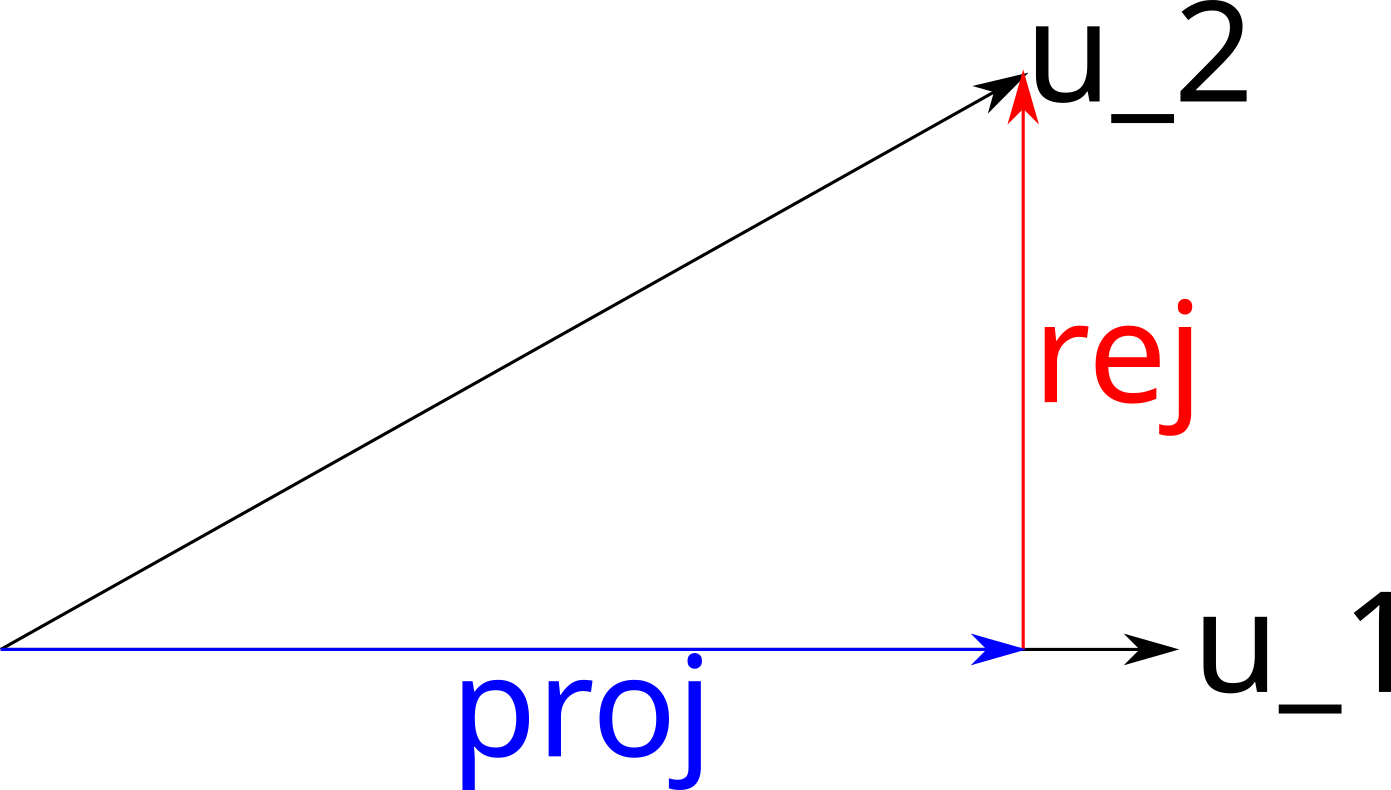
\includegraphics[scale=0.50]{./Vector_Projection_Rejection.png}
  \caption{Vector Projection and Rejection}
  \label{fig:Vector_Projection_Rejection}
\end{figure}

\begin{theorem}[Gram-Schmidt Orthogonalization Process]\label{thm:Gram-Schmidt_Orthogonalization}
  Given $m$ \nameref{def:Linearly_Independent} vectors in $\RealNumbers^{n}$ ($m$ vectors, each with $n$ components),
  \begin{equation*}
    S = \lbrace u_{1}, u_{2}, \ldots, u_{m} \rbrace, \: n \geq m
  \end{equation*}

  To find $V = \lbrace v_{1}, v_{2}, \ldots, v_{m} \rbrace$ orthogonal vectors where $\Span(V) = \Span(S)$.

  We can find such vectors by repeatedly using the \nameref{def:Vector_Rejection} of the original vector from the first orthogonal vector.
  So, the process boils down to:
  \begin{equation}\label{eq:Gram-Schmidt_Orthogonalization}
    \begin{aligned}
      v_{1} &= u_{1} \\
      v_{2} &= u_{2} - \Rej{u_{2}}{v_{1}} \\
      &= u_{2} - \frac{u_{2} \cdot v_{1}}{v_{1} \cdot v_{1}} v_{1} \\
      v_{3} &= u_{3} - \frac{u_{3} \cdot v_{1}}{v_{1} \cdot v_{1}} v_{1} - \frac{u_{3} \cdot v_{2}}{v_{2} \cdot v_{2}} v_{2} \\
      &\vdots \\
      v_{m} &= u_{m} - \frac{u_{m} \cdot v_{1}}{v_{1} \cdot v_{1}} v_{1} - \cdots - \frac{u_{m} \cdot v_{m-1}}{v_{m-1} \cdot v_{m-1}} v_{m-1}
    \end{aligned}
  \end{equation}
\end{theorem}

\begin{example}[Lecture 21, Example 1]{Find Orthogonal Vector}
  Given three vectors in $\RealNumbers^{4}$, find $\lbrace v_{1}, v_{2}, v_{3} \rbrace$ where each element is mutually orthogonal, and the \nameref{def:Span} $\Span(S)$ remains the same.
  \begin{equation*}
    S = \lbrace (1, 2, -1, 2), (2, 3, -1, 1), (0, 2, -1, 4) \rbrace
  \end{equation*}
  \tcblower{}
  From \nameref{thm:Gram-Schmidt_Orthogonalization} (\Cref{eq:Gram-Schmidt_Orthogonalization}), we already know how to solve this.
  \begin{align*}
    v_{1} &= u_{1} \\
          &= (1, 2, -1, 2)
  \end{align*}

  Now, we can solve for the second orthogonal vector.
  \begin{align*}
    v_{2} &= u_{2} - \frac{u_{2} \cdot v_{1}}{v_{1} \cdot v_{1}} v_{1} \\
          &= u_{2} - \frac{(2, 3, -1, 1) \cdot (1, 2, -1, 1)}{(1, 2, -1, 1) \cdot (1, 2, -1, 1)} v_{1} \\
          &= u_{2} - \frac{2 + 6 + 1 + 2}{1 + 4 + 1 + 4} v_{1} \\
          &= (2, 3, -1, 1) - \frac{11}{10} (1, 2, -1, 2) \\
          &= \frac{(20, 30, -10, 10) - 11 (1, 2, -1, 2)}{10} \\
    v_{2} &= (\frac{9}{10}, \frac{8}{10}, \frac{1}{10}, \frac{-12}{10}) \\
    \intertext{The scaling is unimportant here, so we can actually drop the fractional part.}
    v_{2} &= (9, 8, 1, -12)
  \end{align*}

  Lastly, we solve for the last orthogonal vector.
  \begin{align*}
    v_{3} &= u_{3} - \frac{u_{3} \cdot v_{1}}{v_{1} \cdot v_{1}} v_{1} - \frac{u_{3} \cdot v_{2}}{v_{2} \cdot v_{2}} \\
          &= u_{3} - \frac{(0, 2, -1, 4) \cdot (1, 2, -1, 2)}{10} v_{1} - \frac{(0, 2, -1, 4) \cdot (9, 8, 1, -12)}{(9,8,1,-12) \cdot (9,8,1,-12)} v_{2} \\
          &= u_{3} - \frac{0+4+1+8}{10} v_{1} - \frac{-33}{290} v_{2} \\
          &= (0, 2, -1, 4) - \frac{13}{10}(1,2,-1,2) + \frac{33}{290} (9, 8, 1, -12) \\
    v_{3} &= (\frac{-8}{29}, \frac{9}{29}, \frac{12}{29}, \frac{1}{29}) \\
    \intertext{The scaling is unimportant.}
    v_{3} &= (-8, 9, 12, 1)
  \end{align*}
\end{example}

\begin{example}[Lecture 21, Example 2]{Gram-Schmidt on Matrices}
  Given the \nameref{def:Real_Symmetric_Matrix} $A$, determine an \nameref{def:Orthogonal_Matrix} that implements a \nameref{def:Diagonalization}.
  \begin{equation*}
    A =
    \begin{pmatrix}
      3 & 2 & 4 \\
      2 & 0 & 2 \\
      4 & 2 & 3
    \end{pmatrix}
  \end{equation*}
  \tcblower{}
  Start by finding the \nameref{def:Eigenvalue}s, and then the \nameref{def:Eigenvector}s.
  \begin{align*}
    A - \lambda I &=
                    \begin{pmatrix}
                      3 - \lambda & 2 & 4 \\
                      2 & 0 - \lambda & 2 \\
                      4 & 2 & 3 - \lambda
                    \end{pmatrix} \\
    \intertext{We can make finding the \nameref{def:Determinant} easier by performing some \nameref{def:Elementary_Column_Op}s.
    Refer back to \Cref{subsubsec:Create_0s_Determinants} for how these affect the determinant's outcome.}
    &\grstep{-2c_{2} + c_{3}}
      \begin{pmatrix}
        3 - \lambda & 2 & 0 \\
        2 & - \lambda & 2 + 2 \lambda \\
        4 & 2 & -1 - \lambda
      \end{pmatrix} \\
    \det(A - \lambda I) &= (1 + \lambda) \det
                          \begin{pmatrix}
                            3 - \lambda & 2 & 0 \\
                            2 & -\lambda & 2 \\
                            4 & 2 & -1
                          \end{pmatrix} \\
    \intertext{Finding the \nameref{def:Determinant} by expanding the first row.}
                  &= (1 + \lambda) \bigl( (3-\lambda) (\lambda - 4) - 2(-2 - 8) \bigr) \\
                  &= (1 + \lambda) (3\lambda - \lambda^{2} + 4 \lambda - 12 + 20) \\
                  &= (1 + \lambda) (-\lambda^{2} + 7\lambda + 8) \\
                  &= (1 + \lambda) (\lambda + 1) (-\lambda + 8)
  \end{align*}
  We get \nameref{def:Eigenvalue}s if and only if $\det(A - \lambda I) = 0$.
  So, we have two \textbf{distinct} eigenvalues:
  \begin{description}[noitemsep]
  \item[$\lambda = -1$] With algebraic multiplicity 2.
  \item[$\lambda = 8$] With algebraic multiplicity 1.
  \end{description}

  Now, finding the \nameref{def:Eigenvector}s. \\
  For $\lambda = -1$:
  \begin{align*}
    \begin{pmatrix}
      4 & 2 & 4 \\
      2 & 1 & 2 \\
      4 & 2 & 4
    \end{pmatrix}
              \begin{pmatrix}
      x_{1} \\ x_{2} \\ x_{3}
    \end{pmatrix} &=
                    \begin{pmatrix}
                      0 \\ 0 \\ 0
                    \end{pmatrix} \\
    \grstep{\substack{-2r_{2} + r_{1} \\ -2r_{2} + r_{3}}}
    \begin{pmatrix}
      0 & 0 & 0 \\
      2 & 1 & 2 \\
      0 & 0 & 0
    \end{pmatrix}
              \begin{pmatrix}
                x_{1} \\ x_{2} \\ x_{3}
              \end{pmatrix} &=
                              \begin{pmatrix}
                                0 \\ 0 \\ 0
                              \end{pmatrix} \\
    \intertext{Convert to system of linear equations.}
    2x_{1} + x_{2} + 2x_{3} &= 0 \\
    \intertext{Solve the system.}
    x_{1} &= \frac{-1}{2} x_{2} - x_{3} \\
    x_{2} &= x_{2} \\
    x_{3} &= x_{3}
  \end{align*}

  So, the \nameref{def:Eigenvector} for $\lambda = -1$ is:
  \begin{align*}
    \begin{pmatrix}
      x_{1} \\ x_{2} \\ x_{3}
    \end{pmatrix} &=
                    \begin{pmatrix}
                      \frac{-1}{2} x_{2} - x_{3} \\ x_{2} \\ x_{3}
                    \end{pmatrix} \\
    &= x_{2}
      \begin{pmatrix}
        \frac{-1}{2} \\ 1 \\ 0
      \end{pmatrix} + x_{3}
    \begin{pmatrix}
      -1 \\ 0 \\ 1
    \end{pmatrix} \\
    \intertext{Where $x_{2} \neq 0$ and $x_{3} \neq 0$ simultaneously.}
  \end{align*}

  For $\lambda = -1$, we have two \nameref{def:Eigenvector}s, but they are not distinct.

  For $\lambda = 8$:
  \begin{align*}
    \begin{pmatrix}
      -5 & 2 & 4 \\
      2 & -8 & 2 \\
      4 & 2 & -5
    \end{pmatrix}
              \begin{pmatrix}
      x_{1} \\ x_{2} \\ x_{3}
    \end{pmatrix} &=
                    \begin{pmatrix}
                      0 \\ 0 \\ 0
                    \end{pmatrix} \\
    \grstep{r_{3} + r_{1}}
    \begin{pmatrix}
      -1 & 4 & -1 \\
      2 & -8 & 2 \\
      4 & 2 & -5
    \end{pmatrix}
              \begin{pmatrix}
                x_{1} \\ x_{2} \\ x_{3}
              \end{pmatrix} &=
                              \begin{pmatrix}
                                0 \\ 0 \\ 0
                              \end{pmatrix} \\
    \grstep{\substack{2r_{1} + r_{2} \\ 4r_{1} + r_{3}}}
    \begin{pmatrix}
      -1 & 4 & -1 \\
      0 & 0 & 0 \\
      0 & 18 & -9
    \end{pmatrix}
              \begin{pmatrix}
                x_{1} \\ x_{2} \\ x_{3}
              \end{pmatrix} &=
                              \begin{pmatrix}
                                0 \\ 0 \\ 0
                              \end{pmatrix} \\
    \intertext{Convert to system of linear equations.}
    -x_{1} + 4x_{2} - x_{3} &= 0 \\
    18x_{2} - 9x_{3} &= 0 \\
    \intertext{Solve the system.}
    x_{3} &= 2x_{2} \\
    x_{1} &= 2x_{2} \\
    x_{2} &= x_{2}
  \end{align*}

  So, the \nameref{def:Eigenvector} for $\lambda = 8$ is:
  \begin{align*}
    \begin{pmatrix}
      x_{1} \\ x_{2} \\ x_{3}
    \end{pmatrix} &=
                    \begin{pmatrix}
                      2x_{2} \\ x_{2} \\ 2x_{2}
                    \end{pmatrix} \\
    &= x_{2}
      \begin{pmatrix}
        2 \\ 1 \\ 2
      \end{pmatrix}
    \intertext{Where $x_{2} \neq 0$}
  \end{align*}

  From the gathered \nameref{def:Eigenvector}s, set our vectors to be:
  \begin{align*}
    u_{1} &= (-1, 2, 0) \\
    u_{2} &= (-1, 0, 1) \\
    u_{3} &= (2, 1, 2) \\
    \intertext{Checking if the vectors' orthogonality.}
    u_{1} \cdot u_{2} &= \left( \frac{-1}{2} \right) (-1) + 1 (0) + 0 (1) \\
          &= \frac{1}{2} \\
          &\neq 0 \\
    u_{1} \cdot u_{3} &= 0 \\
    u_{2} \cdot u_{3} &= 0
  \end{align*}

  We can now use \nameref{thm:Gram-Schmidt_Orthogonalization} to find a new set of vectors which \textit{are} orthogonal.
  \begin{align*}
    v_{1} &= u_{1} \\
    v_{1} &= (-1, 2, 0)
  \end{align*}

  Next,
  \begin{align*}
    v_{2} &= u_{2} - \frac{u_{2} \cdot v_{1}}{v_{1} \cdot v_{1}} v_{1} \\
          &= (-1, 0, 1) - \frac{1}{5} (-1, 2, 0) \\
          &= (\frac{-4}{5}, \frac{-2}{5}, 1) \\
          &= (4, 2, -5) \\
  \end{align*}

  Lastly,
  \begin{align*}
    v_{3} &= u_{3} - \frac{u_{3} \cdot v_{1}}{v_{1} \cdot v_{1}} v_{1} - \frac{u_{3} \cdot v_{2}}{v_{2} \cdot v_{2}} v_{2} v_{2} \\
    \intertext{Remember, $u_{3}$ was already orthogonal to $u_{1}$ and $u_{2}$, so it is orthogonal to $v_{1}$ and $v_{2}$ already.}
          &= u_{3} \\
    v_{3} &= (2, 1, 2)
  \end{align*}

  Lastly, we need to normalize each column, to make an \nameref{def:Orthogonal_Matrix}.
  \begin{align*}
    \Magnitude{v_{1}} &= \sqrt{5} \\
    \Magnitude{v_{2}} &= \sqrt{45} \\
    \Magnitude{v_{3}} &= 3
  \end{align*}

  Thus, our \nameref{def:Orthogonal_Matrix}, $Q$ implements a \nameref{def:Diagonalization} of $A$ whose product is $D$.
  \begin{align*}
    Q &=
        \begin{pmatrix}
          \frac{-1}{\sqrt{5}} & \frac{4}{\sqrt{45}} & \frac{2}{3} \\
          \frac{2}{\sqrt{5}} & \frac{2}{\sqrt{45}} & \frac{1}{3} \\
          0 & \frac{-5}{\sqrt{45}} & \frac{2}{3}
        \end{pmatrix} \\
    D &=
        \begin{pmatrix}
          -1 & 0 & 0 \\
          0 & -1 & 0 \\
          0 & 0 & 8
        \end{pmatrix}
  \end{align*}
\end{example}


%%% Local Variables:
%%% mode: latex
%%% TeX-master: "../../Math_333-MatrixAlg_ComplexVars-Reference_Sheet"
%%% End:


%%% Local Variables:
%%% mode: latex
%%% TeX-master: "../Math_333-MatrixAlg_ComplexVars-Reference_Sheet"
%%% End:
